% !TEX encoding = UTF-8 Unicode
% !TEX spellcheck = en-US


% This is the root file of your thesis: thesis.tex
% A line starting with % is a comment. In some cases, I have included a command preceded by a %. You may activate the command by removing the %.

%%===================================
\documentclass[12pt]{report}
\usepackage{ramsstyle}
%%===================================
%Write the various parts of your thesis as separate files and include them into the main file by the command \include{name of included file}. When you compile the LaTeX file, you may choose which subfiles to include by the command

%\includeonly{chapter01,chapter02}

%%===================================
\begin{document}
% !TEX encoding = UTF-8 Unicode
%!TEX root = thesis.tex
% !TEX spellcheck = en-US

%This is the Titlepage
%%=========================================
\thispagestyle{empty}
\mbox{}\\[6pc]
\begin{center}
\Huge{Web and Social Media Security}\\[2pc]

\Large{Emil Volckmar Ry, Jan Lindemann, Fabian Franz, \\ Audun Kjeldaas, Jørgen Ellingsen}\\[1pc]
\large{Desember 2016}\\[2pc]

PROJECT\\
Faculty of Informatics and Media Technology \\
Norwegian University of Science and Technology
\end{center}
\vfill

\noindent Supervisor: Prof. Dr. Bernhard M. Hämmerli

 % This is the titlepage
\setcounter{page}{0}
\pagenumbering{roman}
% !TEX encoding = UTF-8 Unicode
%!TEX root = thesis.tex
% !TEX spellcheck = en-US
%%=========================================
\addcontentsline{toc}{section}{Preface}
\section*{Preface}
Here, you give a brief introduction to your work. What it is (e.g., a Master's thesis in RAMS at NTNU as part of the study program xxx and\ldots), when it was carried out (e.g., during the autumn semester of 2021). If the project has been carried out for a company, you should mention this and also describe the cooperation with the company. You may also describe how the idea to the project was brought up.

You should also specify the assumed background of the readers of this report (who are you writing for).\\[2cm]

\begin{center}
Gj{\o}vik, Desember 2016\\[1pc]
Jørgen Ellingsen
\end{center}
% !TEX encoding = UTF-8 Unicode
%!TEX root = thesis.tex
% !TEX spellcheck = en-US
%%=========================================
\addcontentsline{toc}{section}{Acknowledgment}
\section*{Acknowledgment}
I would like to thank the following persons for their great help during \ldots

If the project has been carried out in cooperation with an external partner (e.g., a company), you should acknowledge the contribution and give thanks to the involved persons.

You should also acknowledge the contributions made by your supervisor(s).

\begin{flushright}
O.N.\\[1pc]
(Your initials)
\end{flushright}
% !TEX encoding = UTF-8 Unicode
%!TEX root = thesis.tex
% !TEX spellcheck = en-US
%%=========================================
\addcontentsline{toc}{section}{Summary and Conclusions}
\section*{Summary and Conclusions}
Here you give a summary of your your work and your results. This is like a management summary and should be written in a clear and easy language, without many difficult terms and without abbreviations. Everything you present here must be treated in more detail in the main report. You should not give any references to the report in the summary -- just explain what you have done and what you have found out. The Summary and Conclusions should be no more than two pages.

You may assume that you have got three minutes to present to the Rector of NTNU  what you have done and what you have found out as part of your thesis. (He is an intelligent person, but does not know much about your field of expertise.)
\tableofcontents
\setcounter{page}{0}
\pagenumbering{arabic}
% !TEX encoding = UTF-8 Unicode
%!TEX root = thesis.tex
% !TEX spellcheck = en-US
%%=========================================
\chapter[Bot Metrics]{Does bots,  make click, text and behavior metrics irrelevant?}


\section{What are bots and how are they used?}
In general, bots are types of software which run automated tasks(which are repetitive and allows for the program to be faster at doing some tasks than what normal humans would be able to. There are many types of bots, for example gaming bots which can be programmed to efficiently react faster than what a human would be able to on certain events in the game, thus making the humans better players. Others examples include auction bots, which hunt for bargains. Ebay went to court in 2000( \cite{Computerworld:Ebay}) in order to stop this type of behavior, the federal courts in turn then decided to block Bidders Edge and their bots from accessing Ebays API. 
\\
\\
Furthermore bots are used to mimic human activity, in for example service applications which appear to be human interaction but is instead a bot which for example tries to "help" you based on keywords. Bots are used in many areas, but are probably most known for their maliciousness in areas such as spam, bandwidth-thiefs, scrapers, worms and viruses as well as as nodes in a larger scale bot-nets is used for example for DDOS. These bots can be part of bigger bot-nets in order to for example generate revenue through for example click fraud. 
%%
\newpage 
%%
In \cite{Observer:FakeTRAF} the problem and its extent is very well described: \begin{quote}
A recent study by comScore found that 54 percent of display ads shown in thousands of campaigns between May 2012 and February 2013 never appeared in front of a human being. Rather, the traffic came from bots. As an advertiser, this would be like buying a billboard you were told was seen by thousands of cars a day only to find out that was because the billboard sat next to the assembly line at a Ford plant. Sure, that’s a lot of cars, but there’s no one in them.
\\
\\
In fact, the system is so broken that, for some publishers, knowingly buying traffic that comes from bots is part of their business model. An anonymous publishing executive, who claimed to be buying up to \$35,000 worth of traffic per day, recently told Digiday that for publishers running an arbitrage model, all that matters is profit; quality of traffic does not factor into the equation.
\newline \mbox{} \hfill \citet{Observer:FakeTRAF}
\end{quote}
This quote from comScore highlights a important point in todays society. How does click metrics influence us, and how are they used? Are they useless, can they be used to measure something even though results most likely have been contaminated? and how does this type of behavior influence the buyers decision? These and some others are the question I will answer during this chapter. 
\\
\\
I will also look into bots in social media, how they interact and how they spread in order to seem like normal users as well as interact as normal users. 


\newpage
\section{What is  social media statistics, and how is it utilized?}
With the rise of social media use, social media marketing got a bigger foothold, allowing marketeers to interact with their buyers to a bigger degree, and it allowed the buyers to interact with their brands. Following this trend, many companies have big social media presences. Social media statistics allows the companies to closely monitor and narrow down their demographic and easily make specific content for a specific demographic. Furthermore, it allows for the company to get free publicity through what is called "organic reach" (getting exposure through users' activity in order to generate more clicks from users' contact) as well as for example paid reach(ads sent to a predefined demographic)
Social media statistics allows for all of this to happen, as \cite{Singh2013} mentions:
\begin{quotation}
Social Media statistics about audience likes and dislikes makes it plausible to employ “push marketing” techniques to target audiences with advertisements that are relevant to their interests. Also, parameters such as click through rates or CTR can further quantify the success (or failure) of an advertising campaign. 
\end{quotation}
This type of push marketing, utilizes the information the users' themselves have provided to the mother service(e.g. Facebook), like for example metadata which gives a certain characteristic which allows them to be targeted by the broad filters which services like e.g. Facebook uses. 
\\
Businesses also utilizes what is called pull marketing, which is a little more subtle, e.g. referrals, social competitions("like and share" and get the \textit{chance} to win X") these methods can generate traction in social media, and be spread by word of mouth. 
\\
\\
But most notably, these types of metrics can be abused by bots, as we will see in the next section. 

\newpage
\subsubsection*{An example of this type of scam}
So what happens to this type of data in a business when bots(self inflicted or otherwise) enter the fray? Depending on how the bot is designed(i.e if its a crawler, adding all friends of friends, it can greatly impact marketing if this bot also uses all metadata(e.g. companies person X likes) in order to obfuscate its true purpose - liking somepage. 
\\
\\
A good real-life example is \cite{Symantec:Narang}, which had a set of inter chained accounts posing as real accounts in order to spread their own links about some dubious dietpills. The accounts stole metadata from real accounts. Instead of using compromised
accounts to tweet spam links, they were using accounts that impersonated brands and
celebrities. Symantec goes on to describe how they defined three types of accounts involved in this scam:
\begin{itemize}
\item {\textbf{Mockingbird}: Used real data from real celebrities for impersonating these individuals}
\item{\textbf{Parrot}: Fake accounts using stolen tweets and photographs of real women}
\item{\textbf{Egg}: New users with no set avatar}
\end{itemize}

Mockingbirds have the goal of promoting the weight loss tricks. These mockingbird-tweets would get thousands of likes from Parrot-accounts which spiders through the real accounts of the mockingbirds. Parrots then follow any and everyone in the hope that users will follow them back because they are using avatars of attractive women, a tactic that has proven very efficient. The Parrots have real content that they post each day which is fake, an not only the content of the Mockingbird, in order to seem more real. These tweets are usually stolen from real accounts in order to seem real.  The parrots will also engage in discussions and post "reviews" of the diet pills in order to make the diet pills seem more real while the egg accounts just inflate the like counts in order to make the mockingbirds as well as the parrots seem trustworthy. The egg accounts do not post any content, they just follow parrots.
\\
\\ The link provided by the mockingbirds seem real(with pictures of famous people). When a customer orders a free trial, they register the credit card and subsequently lose their money. 


% !TEX encoding = UTF-8 Unicode
%!TEX root = thesis.tex
% !TEX spellcheck = en-US
%%=========================================
\newpage
\chapter{Approaches for Detecting Robots \\ in Social Media}

\section*{Management Summary}
Social media platforms, like Twitter or Facebook, are a vital part of the Internet of today. Social bots are programs, that automatically take actions on those platforms. Among other things, they are used for a variety of attacks that, for example, aim to simulate a broad natural support for an entity or to cover unpleasant facts or opinions. Because of that, the detection of malicious social bots is an important task.

This chapter focuses on approaches that can be used in order to detect social bots. These approaches can be classified in social network based, crowd-sourcing based and feature based. Each of these classes is discussed in detail.

Social network based approaches model the social media platform into a graph that describes the relationships between all users. Based on those relationships they try to decide whether a user is a bot or a legitimate user.
Crowd-sourcing based approaches leverage the social competence of actual humans to decide whether a given user is a bot or not. The decision is based on all visible actions of a user. 
Approaches that are feature based make use of machine learning, where a system is trained with known data. During this learning phase, it analyzes which features of user activity indicate a real user or a bot. Afterwards, it uses this knowledge to decide on real data.

It is found, that all approaches have their weaknesses and problems. In order to overcome these, it is advisable to combine different approaches. In addition, it is important to conduct further research in this topic, since the number of social bots is to be expected to continue growing. Also, the developers of social bots will develop more and more sophisticated methods to make their bots appear human and defenders should be prepared for this. 


\newpage
\section{Introduction}
Social media is an important part of today's Internet.  Of the approximately 3.4 billion internet users, about 2.3 billion, that means almost 70 percent, use social media actively \cite{insight}. Especially in order to obtain information about events and the like, social media is often irreplaceable.  For some people social media platforms even substitute real life personal contact to a large degree.

With this importance of social media platforms in the lives of so many people, they get more and more interesting for people that want to benefit economically from them. These are for example companies that want to promote their products and services via social channels. However, the problem here is that, due to their size, it is hard to disseminate a certain message on social media platforms. Like in many other areas of today's  information technology, big data is a huge topic in social media.

This is one of the reasons, why social robots, in the form as we know them today, have been developed. As software robots are often simply called bots, we will use the term social bot or simply bot in the following synonymously for social robot. The propagation of such bots has reached a remarkable high level. In 2014, the social media platform Twitter stated in a report to the United States Securities and Exchange Commission that up to 8.5\% of their active user base may be social bots\cite{twitterbot}.  We will see in the upcoming chapters, that they are used to spread certain messages, to hide others or simply to give the impression of a much bigger support for a person, thing or belief than there actually is. Social bots are also used to directly attack other, actual users, for example to steal their personal data.

First of all, we will take a look at the definition and history of social bots, in order to clearly define what we are talking about and where it originates from. We will then introduce the online social media platforms that are important for this chapter, namely Twitter, Facebook and Renren, and give a short overview about their characteristics relevant here. Afterwards, we will motivate why social bot detection is actually important. In the main part of this chapter, we will introduce several social bot detection approaches and give examples for them. In the last section we will finally summarize our findings and give an outlook about the further developments in this area.

%	\item https://sysomos.com/inside-twitter/most-active-twitter-user-data 32\% of tweets by bots!

\section{Definition and History of Social Bots} 
This section will introduce the term social bot formally and give a short overview about the beginning and the development of this topic.

In order to be able to discuss social media bot detection, we need a clear understanding of what social bots actually are.  For that, we use the definition given by Ferrara et al. in their article The Rise of Social Bots:
\begin{quote}
	"A social bot is a computer algorithm that automatically produces content and interacts with humans on social media, trying to emulate and possibly alter their behavior." \cite{ferrara15}
\end{quote}

A social bot is therefore basically any software that acts as a user, or something similar, on social media platforms. As the broad definition suggests, they can appear in many shapes.

The root of of social bots, can be found in the Turing test, developed by Alan Turing in 1950 \cite{turing}. It involves three parties, two of them are human and one is a computer program. While one human is having a conversation with the software, it is the task of the other human to identify the program by looking only at the conversation. If he is not able to do so, the software is passing the Turing test. This led to the development of a lot of so called chatbots, which just aimed to appear as human as possible in a conversation.  

A rather famous and often cited example for such a chatbot is ELIZA, introduced by Joseph Weizenbaum in \cite{eliza}. It mimicked a psychotherapist and showed that, at least some kind  of, communication between a human and a computer is possible.

Since then, a lot of things have changed. Today, bots are a lot more than bare entertainment or proof of concept. With the triumph of the Internet and especially social networks like Facebook and Twitter, the possible use cases for social bots have increased dramatically. While they were initially mostly used to simply post content, today they are able to credibly interact with each other and even humans \cite{boshmaf13, hwang12}. As we will see in the next section, nowadays' bots are used to spread messages, for marketing and a lot more.

\section{Important Social Media Platforms}

In this section we want to give a short overview about the social media platforms, or online social networks (OSNs), that are relevant for this chapter. This is necessary in order to better understand the problems and attacks that will be presented later on. However, we will describe those networks only as detailed as necessary in this context, since a thorough explanation would go beyond the scope of this chapter.

The first and probably most important OSN that needs to be mentioned here is Twitter\footnote{https://twitter.com/}. Twitter is a microblogging network which allows its users to broadcast short messages, so called tweets. Tweets are delivered to anyone that follows the tweeting account. Following is hereby a one-way process, that does not need any confirmation by the followed account. To see the tweets of a certain account, following is not necessary though. Thus, tweets can be regarded as public. Furthermore, tweets can be retweeted. Retweets can be seen as a forwarding of a tweet in order to disseminate it: all followers of the retweeting account get the retweeted message.  Tweets can be tagged with hashtags, that associate them with a certain topic or an ongoing discussion.

Another OSN that is important for this chapter is Facebook\footnote{https://www.facebook.com/}. As on Twitter, it is possible to publish messages on Facebook. However, the visibility of those messages, or posts, can be adjusted. Usually, posts are only visible to users that are friends with the posting account. A friendship is here, in contrast to follow-relationship on twitter, bilateral: a user can send a friendship request to another account which has to accept it in order for the relationship to be built. Another important difference to Twitter is, that Facebook accounts respectively profiles usually contain a lot more personal information than Twitter accounts do. Like it was the case with posts, the visibility of Facebook profile pages can be adjusted and usually they are only visible to accounts that are friends.

The last platform we want to mention shortly is Renren\footnote{http://renren.com}, which is a chinese OSN directed mainly at college students. Like Facebook it uses the concept of friendships and highly personalized profiles. It also allows to post messages that can be seen by friends.

\section{Why is Bot Detection in Social Media Important?}
Another point that is important to be looked at before we go into detail about the actual detection methods is, why social media bot detection is important at all. In this section we will argue, why this is an important topic, especially today. 

As already said above, social media platforms are nowadays an important component in the life of many people. For some, they even substitute real personal contact sometimes. Thus, it is important to ensure, that humans are still able to estimate what is happening in their social media surrounding and what can be seen as trustworthy -- and what cannot. While the challenge of verifying facts or news from the Internet is not new, social bots add a new factor to this challenge. They can make a non-trustworthy source look trustworthy by simulating that it is highly popular.

An example for this, is the so called astroturfing. In an astroturfing campaign, an attacker tries to give the impression of a broad grassroot support for a certain person, belief or political position. A known political astroturfing case are for example the 2010 Massachusetts senate elections in the US. During these, a small number of Twitter social bot accounts produced a large amount of tweets that contained a link to a website that smeared one of the candidates. The tweets also mentioned users that had shown the same political position beforehand and thus were likely to retweet. In a few hours the smearing website link spread rapidly what was even noticed by the Google search engine. That way, the website got promoted to the top search results for the name of the smeared candidate \cite{mustafaraj10}. 

A similar approach can also be used to distract from potentially inconvenient or just unwanted facts or opinions is called smoke screening. By just flooding the platform with information, it aims to draw attention away from the unwanted topic to a topic that suits the attacker more. The flooding information can hereby even be related to the topic that is to be screened. It just focuses on a component that is more pleasant to the attacker and withholds the inconvenient part. An example for this is given by Abokhodair et al. \cite{abokhodair} in the context of the syrian civial war. They analyzed a social botnet on Twitter from April until December 2012. It made heavy use of this technique in order to cover up news about the civil war in Syria.

Another, more direct, example for an attack scenario is described by Boshmaf et al. \cite{boshmaf13} They operated a network of social bots on the social media platform Facebook and successfully tried to build as many relationships as possible with real users. After this was done, they were able to extract data from the profiles of those real users that were not publicly available, like for example mail addresses or phone numbers. While they show that operating such a botnet for the sole purpose of data extraction might not be efficient for an attacker, they argue that this data can be used for more advanced attacks afterwards.

Besides all these specific attacks, which are carried out by bots built for this purpose, there are also simple negative effects from social bots that have not necessarily been built for an attacking purpose.
The information in social media is often used by various entities. An example for this is the area of emergency response. By analyzing the information streams of social media platforms it is possible to estimate emergency situations and to take proper actions for decision makers. Cassa et al. \cite{cassa} for example show, that information about the Boston Marathon attacks in 2013 was more than five minutes earlier available on Twitter than the public health alerts, even though there were already many first responders present on this event.  Another area where information from social media platforms is leveraged is the stock market. By monitoring the general mood on Twitter, for example, it is possible to predict the market trend to a certain degree \cite{bollen}. A case can be made that this is also already done by traders. When in 2013 for example the Twitter account of the Associate Press was hacked and it posted rumors about a terrorist attack, the stock market crashed significantly \cite{ferrara15}. It is therefore not hard to see that bot-caused information distortion on social media platforms -- that does not even necessarily needs to be intended malicious -- can have severe impact. Some social bots are built just to retweet and if they retweet false information or rumors they help to make this information popular. This happened for example also after the former mentioned Boston Marathon attacks, where false accusations were spread by such social bots \cite{gupta}. 

Furthermore, social bots are often used by public persons in order to appear more popular and thus to gain influence or by companies in order to promote their products on social media platforms \cite{stringhini}. Here, social bot detection is necessary for ordinary users as well to be able to distinguish between real and bought support.

%---> section "engineered social tampering" and following in the rise of social bots!! 

%\textbf{Im Prinzip angriffsübersicht?}

%+ Key Challenges in Defending Against Malicious Socialbots \cite{boshmaf12}


\section{Social Bot Detection Approaches}
In this chapter we want to introduce several techniques for detecting social bots. Based on Ferrara et al. \cite{ferrara15} we distinguish three detection approach classes. 

The first category of detection approaches is based on social network information. They are also called graph-based, since they map users and their relations into a graph and then try to identify bots in the hereby obtained social network by means of graph theory. 

Afterwards we will discuss crowd-sourcing based social bot detection approaches. They use actual humans to detect bots, assuming that the human ability to notice details in communication will make this an easy task.

The last category we want to elaborate on are detection approaches based on behavioral features. Mechanisms that make use of this approach try to observe behavioral patterns that are typical for humans and social bots. By doing so they aim to distinguish bots from human users. 

In the following sub sections, we will go into detail about each of these three approaches and illustrate them using real detection systems. It has to be noted though, that the borders between the individual approaches is not always very clear, so that some examples could also be mentioned in a different category. Many schemes for example, use some kind of graph theory. However, we try to categorize them by their core traits.

\subsection{Based on Social Network Information}
A term that is often used in combination with detection of bots by using social networks is sybil or the sybil attack. It was presented as a thread to distributed systems by John R. Douceur \cite{sybil}. In the specific context of social media platforms, when conducting a sybil attack, an attacker creates a large amount of fake identities in a system to the point where these identities make up a considerable fraction of the system's whole user base. When this is achieved, the attacker can influence the whole system and control its contents to a certain degree. A sybil, sybil node or sybil account is therefore simply one of the fake entities, or depending on the attack's architecture, just a social bot. It is not hard to see that social bot detection can, more specifically, be viewed as a defense against the sybil attack.   

The general proceeding of bot detection approaches based on social network is rather simple. They map the user base of the OSN they aim to defend into a social graph, where a node is corresponding to a user and an edge between two nodes exists if there is a specific kind of relationships between the two respective users on the platform. The nodes can hereby be distinguished in sybil nodes, respectively bots, and non-sybil nodes, respectively legitimate users. The goal of the detection approach is now, to identify whether a given node is a sybil or not \cite{comparison}.

There are a number of proposed social network based sybil detection schemes like for example SybilGuard \cite{sybilguard}, SybilInfer \cite{sybilinfer} or SumUp \cite{sumup}. While they all have different assumptions and use varying algorithms to achieve their goal, Viswanath et al. \cite{comparison} show that, at a high level, all of them work by them same principles.

Basically they can be viewed as graph partitioning algorithms, which partition a given graph into multiple disjoint subgraphs. As already mentioned above, ideally two subgraphs are assembled, one that contains only sybil nodes and one that contains only non-sybil nodes. Since a clear distinction is often hard to make, the approaches basically assign a rank to each node and decide afterwards, depending on several parameters, which ranks are classified as sybil and which as non-sybil. It is thus obvious, that the ranking algorithm is crucial for the whole scheme. Although, of course, the ranking algorithms for the different detection schemes are different, they generally have in common, that they base their rating on how tightly connected the respective node is to a known trusted node. Thus, they work by detecting local communities of nodes, in other words closely connected groups of nodes \cite{comparison}.

It is not hard to see, that these algorithms are therefore easy to deceive. If an attacker is able to establish so called attack edges, connections between his sybil nodes and non-sybil nodes which are connected to a trusted community, it gets significantly harder to identify the bots. A common assumption is that these attack edges are hard to create \cite{sybilguard}, which means, that legitimate users tend to not establish social network connections to social bots. However, Boshmaf et al. show \cite{boshmaf11} that this assumption is to be questioned. 
They tried to infiltrate Facebook with a large number of sybil accounts and to establish connections to real users. The average acceptance rate of their friendship requests came to about 20\% and could be increased to 80\% depending on how many indirect friendships between the sybil and the user already existed \cite{boshmaf11}.

A well known example for a bot detection approach that is based on social network information is the Facebook Immune System (IMS) \cite{fis}. This system aims to defend the social media platform Facebook and its users not only against sybil attacks but also to prevent spam, malware distribution, phishing and so on.  To achieve this goal, it takes a lot more actions than the above described general approach for social network based detection schemes. The IMS runs checks on every action performed on Facebook in realtime in order to give attackers as less time as possible to accomplish their goals and to react. It classifies these actions according to predefined policies and makes it thereby possible to judge them and the corresponding users.

An example for this could be a newly created Facebook account, that sends a lot of friendship requests. A legitimate user starts sending friendship requests usually mainly to people he knows and vice versa, that is, people that are likely to accept his friendship request. If a lot of these requests are now declined, this could be a indication for the system that the sending user might not be legitimate.  The IMS also makes heavy use of machine learning, to which we will come back in later on, and generates training data automatically in order to adapt to the fast changing attacks and user behavior.

\subsection{Based on Crowd-Sourcing}
A rather straight forward approach for social bot detection is based on crowd-sourcing. In contrast to the above described social network information based approaches, a connection between bots and legitimate users is not a problem for schemes based on this approach -- at least not a direct one. The basic idea of crowd-sourcing based social bot detection is, to engage actual human workers to study user profiles and subsequently to decide whether it belongs to an actual user or a sybil.

Wang et al. \cite{wangcrowd} present a study on the effectiveness of this approach and introduce a sample for a crowd-sourcing based social bot detection system.  For their tests they use data from Renren, China's most popular social media platform, Facebook US and Facebook India. They subdivide their human investigators, or simply testers, in expert workers, and crowd-sourced workers.  Each of the testers is presented a number of social media profiles and has to decide, whether it is a real one, or a sybil. While the experts achieve a detection rate at about 90\%, the crowd-sourced workers perform not as well individually. If their single votes are aggregated and used for a majority decision though, the results can be significantly increased. If this is done for the expert workers, their results can be increased even more, too. A very desirable result of their studies is also that the false positive rate, that is the amount of profiles that are falsely classified as sybils, is in all groups very close to zero. This ensures, that the probability that legitimate users are accused to be social bots, what will probably offend them, is very low.

Wang et al. conclude, that it is very hard for sybil creators, to assemble social bots, respectively profiles, that are able to pass a "social turing test" and that crowd-sourcing based approaches can perform very well. They proceed with introducing a general practical system that is illustrated in figure \ref{crowdsys} \footnote{Turkers are in this case the former mentioned crowd-sourced workers.}.

\begin{figure}
	\centering
	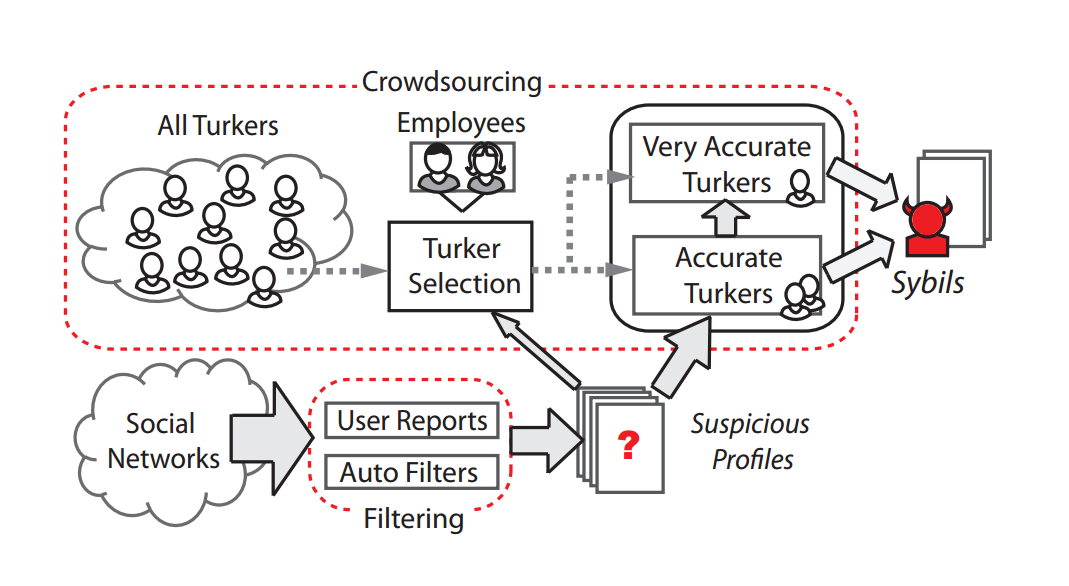
\includegraphics[scale=0.4]{fig/crowdsys}
	\caption{A crowd-sourced sybil detection system introduced by Wang et al. \cite{wangcrowd}.}
	\label{crowdsys}
\end{figure}

The system works like this: The social network that is to be defended generates suspicious profiles. This can either happen through explicit reports from users or through automatically applied filters that detect abnormal behavior. The so obtained profiles are then checked by crowd-sourced workers, which are subdivided in accurate and very accurate. To establish this differentiation, some of the suspicious profiles are mixed with some profiles that are known to be sybils. They are presented to all workers and their results allow a classification and to filter out unreliable workers. In the actual checking process, the profiles are first presented to the accurate workers which make a majority vote. If their decision is not clear, the profiles are presented to the very accurate workers which once again make a majority vote. 
The authors claim, that a system like this is very reliable and cost effective. 

Although such a social bot detection approach based on crowd-sourcing seems very promising at first sight, several problems become obvious on closer examination. First of all, this approach works optimal if every newly created profile can be reviewed in the above described way. However, young social media platforms will probably not be able or willing to pay for this bot detection scheme. A factor that may influence this could also be, that those platforms probably do not have huge issues with the social bot problem in their early stages. Once the platform has grown and the issue arises though, their is usually already a huge user base that has to be reviewed retrospectively. This is not optimal and may take a considerable amount of time.

Another point that must be taken into consideration is that this approach might not be suitable for all types of social media platforms. While it might be well suited for platforms like Facebook or Renren, where profile pages can be customized a lot and contain usually plenty of information, other networks, like for example Twitter could be less appropriate for this approach. Generally it can be said that this detection approach is highly based on the information given in the users' profiles. If the information contained in the profiles is low, human investigators will probably not be able to distinguish as precisely as in the tests of Wang et al.

The last and probably most difficult issue that has to be mentioned is connected to this. Human investigators that are charged with distinguishing between bots and legitimate users need to have access to the profiles of the users. While those profiles are sometimes publicly available anyways, detailed profiles, which are more interesting for this approach, are, as discussed above, usually only visible for certain users. It is not hard to see the privacy issue that arises here, especially when keeping in mind, that the investigators are -- at least to a great extent -- only crowd-sourced workers, that cannot be supervised as easily as ordinary employees \cite{ferrara15}.


\subsection{Based on Features}
The last detection approach for social bots is based on features. Features hereby mean observable characteristics of posted information, profiles and possibly anything else that can be associated to the account in question. Schemes that make use of this approach often use machine learning algorithms. These are algorithms that are able to make decisions based on learned patterns. They basically consist of two phases. In the first phase, the so called training phase, the algorithm processes training data which is labeled with the decision that should be made on this piece of data. By processing a lot of training data, the algorithm learns the features that are indicators for a certain decision. In the second phase, real data is processed and the algorithm is able to make decisions based on the learned data. Thus, schemes that make use of this detection approach can be compared to anomaly based intrusion detection systems. In the social bot detection topic, the decision being made is usually whether a specific account is controlled by a bot or a human. Since it is not easy to make a clear decision in many cases, there are often multiple decision options that each express a degree of certainty.

A well known example for this kind of social bot detection is the Bot or Not? system, presented by Davis et al. \cite{botornot}. It is a publicly available\footnote{http://truthy.indiana.edu/botornot} system that allows a feature based social bot detection for accounts on the social media platform Twitter. Bot or Not? was trained with about 31000 account samples of both, human and social bot accounts. For classification, it makes use of more than 1000 features that can be assigned to six feature-classes. In the following we want to mention these classes shortly:
\begin{itemize}
	\item \textbf{Network} features reflect on the spreading of information, for example citations of different users or the like.
	\item \textbf{User} features take the information given in the actual account into consideration. Meta-data, that is basically data about data, is especially relevant in this feature. 
	\item \textbf{Friends} features are about the social relationships of the account in question.
	\item \textbf{Temporal} features analyze issues like the rate in which content is produced and the like.
	\item \textbf{Content} features are about wording characteristics in the texts produced by the relevant account.
	\item \textbf{Sentiment} features reflect on emotional aspects and are obtained by using specific algorithms \cite{botornot}.
\end{itemize}  
If a Twitter account name is entered in the Bot or Not? system, it checks all of those features and afterwards decides, based on the former mentioned training data, whether this account is a human or bot account.

Another social bot detection approach that can be classified as, feature based relies on detecting the coordinated behavior between social bots. Schemes that make use of this approach focus generally on the above described network, content and temporal features and often incorporate some graph theory as well. They usually aim at detecting attacks which try to distract from unpleasant facts or to distribute fake facts, like in the above described astroturf attack.  An example for such a scheme is SynchroTrap, presented by Cao et al.  \cite{synchrotrap}. Again, comparable to anomaly based intrusion detection systems, SynchroTrap makes use of clustering algorithms. These algorithms try to group values, that are similar in some aspects into distinct sets. 

The system monitors all user activity on a social media platform over an extended time period and monitors aggregated user actions. Then, the pairwise similarity between actions is determined and a hierarchical clustering algorithm is used to group users that show similar behavior at approximately the same time. If a cluster is growing too big, it can be assumed as malicious, since legitimate users tend to behave diverse \cite{synchrotrap}.

An issue of this detection method is though, that it is for example not able to detect bot accounts that show a mixture of bot and human behavior. Thus, the detection systems have to be developed further in order to keep up with the fast evolving social bots and their evermore sophisticated behavior \cite{ferrara15}.


\section{Summary and Outlook}
In this chapter, we firstly introduced the term social bot, defined it and looked at the history of robots in social media.  We also gave a really short overview about the OSNs that are most important for this chapter and motivated why social bot detection is important after all. Mainly, we discussed social bot detection approaches. We distinguished hereby social network information based, crowd-sourcing based and feature based approaches. 

Social network based approaches model the analyzed OSN into a graph where users correspond to the vertices and relationships between the users correspond to the edges of the graph. Afterwards, an algorithm tries to make a decision whether a given node is a social bot or an actual user. A problem these systems have to cope with is, that they tend to assume, that bots can't establish relationships to actual, what emerged to be false.

The basic idea of crowd-sourcing based approaches is, to engage actual humans to analyze given user profiles and to decide whether they belong to an actual user or a social bot. We discussed a paper which analyzes this approach thoroughly and introduces a general practical system. One of the issues this approach has to handle is that some social networks users don't have very detailed profiles what makes crowd-sourced bot detection very hard. 

Feature based social bot detection approaches observe characteristics of OSN users and information published by them in order to decide -- or give a tendency -- whether a given account is a bot or not. Often, they make use of machine learning algorithms. 

After analyzing the different detection approaches, it becomes apparent that each has its own problems and a combination of different approaches may yield good results. Observing the social graph and behavioral features of accounts together is for example a promising strategy. Ferrara et al. \cite{ferrara15} bring in the Renren sybil detector \cite{wang2013, yang2014} as a good example for these combined approaches.

However, it has to be noted that not all robots in social media have to be evil necessarily. Some social bots provide useful services that many users do not want to miss. It is just important, that users are able to distinguish between other humans and bots for example in order to differentiate whether content they see is actually as popular as it seems.

It is safe to assume that the number of social bots will increase even more and that their methods and behaviors will get even more sophisticated. We expect an arms race between bot herders and bot detection mechanisms, like it was -- and still is -- the case with malware and malware detection software.


% !TEX encoding = UTF-8 Unicode
% !TEX root = thesis.tex
% !TEX spellcheck = en-US
%%=========================================
\chapter[Social Media Attacks]{Social Media attacks on mobile devices vs. attacks on computers}
\subsection*{Management summary}
We have seen an enormous increase in online social media in popularity during the past decade. It has taken over a lot of the networking people tended to do in real life earlier and it makes keeping in touch with a larger network of people a less laboursome task. We tend to trust a friend more than we would any random person on the street and this trust mechanism has been transferred to the cyber space. Cybercriminals, who seem to be mostly concerned with gaining wealth, political high ground, or are ideologically motivated, have shown a keen interest in utilizing these new networking platforms. They come from several different directions, such as attacking via vulnerabilities in hardware, OS, protocols, and apps, but they are also successfully exploiting the trust that exists between members of a social network.
In this paper I am looking at the differences between the security topography for social media users, on a mobile device, versus that one would navigate when utilizing a personal computer. I have found quite a few differences and in other areas the situation is quite similar. The conclusion I reached was that it is, at least at present, much safer to use social media on a regular personal computer than on a mobile device, but that it also depends to a great degree how the user behaves security vice. The share of time people spend on social media networks on their mobile device versus on their computer is already 79% vs 21% [11] and still the mobile platform is rapidly gaining terrain. The mobile platforms are getting better protection, but still they are behind on sophistication level when it comes to security. From what I have seen it looks as if you are an easier target for social media attacks when you are using a mobile device than you are doing the same social media networking on your computer.
\section{Hypothesis and methodology}
My hypothesis is that it is easier to attack social media users via their mobile platform gadgets, than via their use of the same media on computers. I have weighed different factors and gathered information around the subject by reading published material saying something about usage pattern, platform weaknesses, distribution of vulnerabilities, and how the users time is divided between the two platform categories. I have looked at how software and hardware protection is being utilized the two cases and I will in the end try to conclude based upon the information presented.
 The subject of social has been moving so quickly, behavioural statistics changing drastically from one year to the next. This constant change makes it difficult to obtain standard peer reviewed research with the latest numbers. For this reason, I have partially leaned on numbers obtained from white papers published by some of the big commercial players in the information security market. These papers are recognized by the industry as reliable sources for such information.
\section{Introduction}
Social media attacks are increasingly common. People’s usage pattern of social media has also changed dramatically during the past few years. An increasing amount of people’s social media interaction is being conducted on mobile hardware platforms. Instead of using Facebook, LinkedIn and other media on the Personal Computer they may or may not still have in their home, they are now using the same media on their mobile devices, such as pads and smartphones. There are also new social media appearing, especially made for these mobile platforms, such as Instagram, which is made to share photos taken with your smartphone on the go.
People now spend more time interacting on social media using their smartphone, than they do using their computer. According to comScore 79% vs 21% [11]. Since this is a relatively new trend, that has exploded in the past couple of years, it is interesting to see if the migration from one platform to another has led to a more unsecure situation for the users. I limit the type of attack here to direct attacks on end users, with the intension to extract either labour, money or personal data. Nevertheless, I think that the result says something about the security difference we currently have between these two types of platforms.
\section{Attacks on social media users in general}
Some of the most popular social media providers today are Facebook, LinkedIn, Twitter, Google+, YouTube, Pinterest, Instagram, Vine, Snapchat and Reddit. There are myriads more and new services pop up all the time.
While using portable devices to access social media, the user is both a possible target for the same types of attacks that we find being used against computer users and at the same time the limited resources of the mobile devices limits the possibility of using the same advanced mechanisms and software to stay safe [4].
Most attacks on the users of these media are economically motivated. There can be different paths to earning money on a social media attack. The reason for an attack can also be politically motivated or even nation state security concerns. I’ll go through a few and compare possibilities on the different platforms.
As the mobile devices gets ever more advanced and the number of apps, protocols and uses seem to rise towards the sky, it is no big surprise that the number of vulnerabilities follows suit as seen in Figure \ref{fig:mobile_vulnerabilities}.
\begin{figure}
\centering
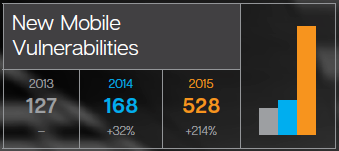
\includegraphics[width=0.5 \textwidth]{fig/mobile_vulnerabilities}
\caption{New mobile device vulnerabilities per year [10].\label{fig:mobile_vulnerabilities}}
\end{figure}
\section{Specific attack vectors for computers}
\subsection{Microsoft Windows}
Microsoft Windows has been the most widely used operating system and thereby represent the largest attackable population. It has also been regarded much easier to attack than the other common computer operating systems, because of the way it is built. 
\subsection{Apple OSX}
Apples operating system was long regarded as the safest choice of operating system for a computer, but 
\subsection{Linux distros}
\section{Specific attack vectors for smartphones}
\subsubsection{Android}
New types of attacks are coming all the time. Cross platform attack on Android is being performed via Google Play in a web browser on an ordinary computer. When the victim logs on to the Google Play account on a computer, to install apps on a mobile device running Android, malware on the computer can steal the browser cookies for that session and use it to impersonate the user. It is then possible for the attacker to remotely install apps on the victim’s Android unit. We can also see that the malware is becoming smarter and the sophistication level is rapidly reaching the level of malware for computers. Example are that they are now both obfuscating the code so as not to be detected by malware protection software that uses signatures, and malware that can check if it is running on a real device or a security company’s emulator, thereby avoiding detection. Another weakness with the Android platform is that even if Google pushes out security patches to the makers of all the different devices as fast as they can, many makers take a long time to push these out to their end users [10].
\subsection{iOS}
Apples screening of apps, before letting them into their App store, is very strict, so one can generally be more trusting towards apps found there. Attackers of Apple’s portable devices, running the iOS operating system, for the most had to rely on finding vulnerabilities or attack a jailbroken device to succeed (unlike Android). This is no longer the case. Several new ways of attacking these devices has recently come to light. Symantec mentions two examples of such attack techniques namely XcodeGhost and YiSpectre which can compromise an iOS device without using vulnerabilities or jailbreaking.
\begin{figure}
\centering
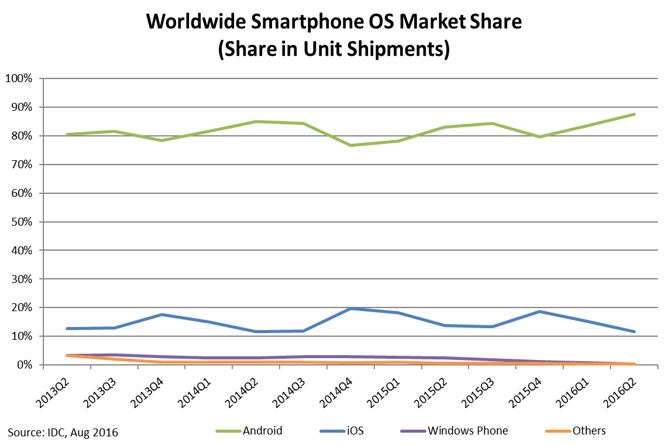
\includegraphics[width=0.8 \textwidth]{fig/smartphone_market_share}
\caption{According to IDC (IDC, Aug 2016) the market share for the Android smartphone OS in August 2016 was 87.6\% And for iOS 11.7\%.\label{fig:smartphone_market_share}}
\end{figure}
The OS distribution in the market means that attackers probably concentrate on Android to get the highest return for their effort. In fact, Kaspersky Lab and INTERPOL has made a report that states that an estimated 98.05% of all malware is coded to target Android. They also found (in 2014) that the number of detected malware programs for Android had almost tripled since the previous year [8]. 
\section{Social media attacks directly on the given platform}
As we have seen there are many ways of attacking social media users/accounts via the platform they are using the media on. There are however a lot of ways to attack via the social media itself, without depending on vulnerabilities in the hardware or software. The attacks simply rely on the many vulnerabilities found in the users, so to speak. These kind of attacks are usually categorized as 
\subsection{User behavioural aspects}
\subsection{Hardware and software}
The way we use these mobile platforms will largely effect how safe we are from attacks. A lot depends on whether the user installs some kind of antivirus/antimalware program on their device and also how the user thinks about security, compare to when using computer.
Many users leave the Wi-Fi on all the time. It is convenient to have your device connect automatically to all the networks you use, but this convenience comes at a high cost security wise. It is increasingly easy to attack these users by setting up a portable “Wi-Fi-box” that answers the unknowing smartphone owner’s device’s call for a named network, saying “Yes, here I am, please connect to me”. Such devices can be bought readymade on the Internet; an example is the Wi-Fi Pineapple (https://www.wifipineapple.com/).
The other radios in the devices, like Bluetooth and NFC, are also possible entry points for an attacker. We have seen attacks lately using NFC-code stickers containing malicious code or pointing the device user to a malicious website. These stickers can be bought for less than a dollar, programmed via a smartphone and printed with for example “Scan to get 100 free Instagram followers” or something to get people to scan it. An example of a possible attack could be to make the sticker point the user to a mock-up web page that looks like Instagram and since they already think they are there to get more followers they wouldn’t react on having to enter their username and password. 
\subsection{Social media network trust}
People build their social networks online, for most, as they do in real life. They either do know or at least feel they know the people in their social media network to a certain extent. This again leads to trust. People tend to trust the people in their social media network, just the way they trust their friends and co-workers’ in real life.
This trust makes the users easy prey to attackers making it look like links and other things has been sent to them by someone in their network. This can be both sent directly as a personal message, shared to all friends or simply liked. The most popular form of social media scam is manual sharing. Manual sharing consists of something that looks great in some way so that users themselves will want to share it with their friends, like for example a cool video or the chance of winning a new car if you share the post.
\begin{figure}
\centering
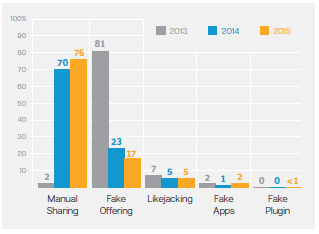
\includegraphics[width=0.5 \textwidth]{fig/social_media_scams}
\caption{Social media network scams by popularity [10].\label{fig:social_media_scams}}
\end{figure}
The mechanisms of these scams works the same regardless of platform, since they are relying on the intended functionality of the app or web page. There should not be any difference in the way people
\section{Conclusion}
Based upon the material I have reviewed I would have to conclude that it is much easier to attack social media users via their portable devices, than it would be to attack their computer. The main considerations behind my conclusion are the following: The majority of time spent on social media is spent accessing these on a mobile device and not a computer. Very few people install any form of malware protection on their mobile devices, while a good majority installs malware protection on their computers. The malware protection solutions that exists for mobile devices, are inferior to the systems available to do the same task on a computer. The number of vulnerabilities found for mobile devices per year is rising quickly. People tend to walk around town with Wi-Fi, Bluetooth, and NFC turned on for anyone to exploit.
So the advice to the general public should be to at least install some sort of malware protection on all their devices, don’t leave Wi-Fi, Bluetooth or NFC on when it is not in use.
% !TEX encoding = UTF-8 Unicode
% !TEX root = thesis.tex
% !TEX spellcheck = en-US
%%=========================================
\chapter[Web Application vulnerabilities in 2016]{Common vulnerabilities and attack surfaces for Web Applications in 2016}

\subsection*{Management summary}
The web stack has evolved to serve feature rich and dynamic experiences within the browser by expanding on the legacy applications. The majority of cyber attacks are done at web application level, and most of the vulnerabilities are well known and documented - but alot of web applications fail to mitigate or counteract them.

This chapter several reports from security companies and non-profit organizations was analyzed to find some of the most common web application vulnerabilities with the possibility of severe consequences. The chapter focuses on Cross-Site Scripting, SQL Injection and vulnerable JavaScript Libraries to explain how they work and how they can harm the companies and their visitors/clients. It briefly looks at the rising usage of Exploit Kits, and how these vulnerabilities can compromize the web application and make it a part of an Exploit Kit infrastructure. It continues to look at possible mitigation techniqes and countermeasurements and discuss why so many sites are vulnerable to these well-known attack surfaces.
%%=========================================
\pagebreak
\section{Introduction}
Over the last years web application hacking has increased, and as many as 75\% of cyber attacks are done at web applications level or via the web \cite{AcunetixCompany}. The introduction in the Acunetix report states that 55\% of web applications has atleast one high-severity vulnerability - and thats up 9\% since 2015.

The web stack has evolved to serve feature rich and dynamic experiences within the browser by expanding on the legacy applications. This has widened the attackers oppertunities, and the amount of vulnerable applications on the web is ever increasing \cite{Acunetix2016}. In recent years an alarming number of high profile web service providers has lost huge amounts of personal data, including emails and weakly hashed passwords. \\ This chapter aims to find the most common vulnerabilities and attack surfaces for web applications in 2016, what the consequences can be, what measures can be taken, and hopefully a hint to why so many web applications are still vulnerable.
\\ \\
This chapter will focus on the application code vulnerabilities that might arise from poor programming and vulnerable third-party libraries in the application itself. A combination of the results of four induvidual information security reports will be examined to find a few vulnerabilities that occur often and are of high severity. Three of the reports are from 2015/2016, and the fourth is OWASP Top 10 from 2013. \textbf{More on methods}
\subsubsection{OWASP Top 10}
Open Web Application Security Project is a international charitable non-profit organization, and is a colaberation between a varity of security experts around the world \cite{OwaspCompany}. The primary aim of the OWASP Top 10 is to raise awareness for web application security, and so far the report has been released twice, in 2010 and 2013 \cite{OwaspTop10Project}.
\subsubsection{Acunetix Web Application Vulnerability Report 2016}
Acunetix is a company spacializing in automated tools to scan servers for vulnerabilities, and have many high profile private and public companies as clients \cite{AcunetixCompany}. They released an annual report on statistics from their scans throughout the period of 1st April 2015 to 31st March 2016. Acunetix has gathered, aggretated and analyzed data from over 61.000 scans over a two year period, and are in a great position to observe trends in the field \cite{Acunetix2016}. 
\subsubsection{Hewlett Packard Enterprise Security Research Cyber Risk Report 2016}
Hewlett Packard provide a broad view of the 2015 threat landscape, based on industry-wide data and a focused look at open source, mobile and IoT \cite{HP2016}.
\subsubsection{Symantec Internet Security Threat Report 2016}
Through the Global Intelligence Network, Symantec has one of the most comprehensive sources of internet threat data \cite{Symantec2016}. It's made up of more than 63.8 million attack sensors in over 157 countries and territories through a combination of Symantec products and services \cite{Symantec2016}.
\pagebreak
\section{Trending vulnerabilities and consequences}
This section will introduce the three common high-severity vulnerabilities that this chapter will focus on. By examinin the reports listed in the Introduction, the choice has fallen on Cross-Site Scripting (XSS), SQL Injections and Vulnerable JavaScript libraries. All of the threats described here have consistently been reported as the most common vulnerabilities in web applications for several years, and 2016 is no different \cite{OWASP2010}\cite{OWASP2013}\cite{Acunetix2016}. They are all vulnerabilities that arise in the development phase of a web application, and they can all potentially cause significant damage. 
\subsection{Cross-Site Scripting (XSS)}
If an attacker is able to submit malicious HTML such as JavaScript to a dynamic web application, they are able to execute a Cross-Site Scripting, or XSS, attack \cite{Kirda2011}. \\
Unlike traditional distributed systems security where access control equals authentication and authorisation, a web application uses the same-origin policy \cite{Gollmann2011}. This policy is exploited by a Cross-Site Scripting attack, when the vulnerable site is viewed by a victim the malicious content seems to come from the trused site, and the attacker can steal cookies, session identefiers and other sensetive information that the web site has access to \cite{Kirda2011}. Cross-Site Scripting can be viewed as two categories, Persistent and Non-persistent attacks. In a persistent attack the attacker is able to store some malicous code in the database or a file that are rendered as part of the website for future visitors \cite{Edmunds2016}. In a non-persistent attack the attacker uses parameters in the url to inject malicious code to the server, potentally deleting or disclosing sensitive information \cite{Edmunds2016}.
\\ \\
Consider the following scenario:
A user connects to \textit{trusted.com} where they are a registered and authenticated user. In \textit{trusted.com/forum} a malicious user has posted a seemingly innocent post, but managed to append some unsanatized JavaScript code at the end of the post. The JavaScript snippet is not visually rendered by the browser, but executed in the background. The JavaScript snippet then sends the cookie of the victim to \textit{malicious.com/save?cookie=} and append the cookie for storage.

A twitter tool called TweetDeck had a serious Cross Site Scripting vulnerability in 2014 that made it possible to tweet unsanitized input \cite{TweetDeck}. This was a self retweeting tweet, with a small red heart as the only visible content. Lets look at the code as it was injected:
\begin{quote}
\fontfamily{cmtt}\selectfont
{$<$script class="xss"$>$\$(`.xss`).parents().eq(1).find(`a`).eq(1).click() \\ ;\$(`[data-action=retweet]`).click();alert(`XXS in TweetDeck`)$<$/script$>$}
\end{quote}
If we examine the code in this attack, it starts out by opening a \textit{script} tag and giving it a css class called \textit{xxs} to be able to use it as an reference. The \$ refers to jQuery, a popular JavaScript Library, and uses the class previously created to locate the parent containers. Then it picks the second parent out of the list of parents, which in this case is the tweet box. It then continues to find all the link tags and again select the second one, which in this case is the retweet button - and clicks it. This in turn opens a popup to confirm the retweet and the next jQuery tag clicks on the comfirm tweet button, or \textit{[data-action=retweet]}. It finally promts the user with a JavaScript alert saying \textit{"XXS in TweetDeck"} and closes off the script tag.

Now this is a fairly innocent attack, and you could argue that this attacker did this to either show of their skills or alert the twitter developers of their error - or even both. There is no reason to alert the user if you want this to go unnoticed as long as possible, so it's safe to assume that this vulnerability could have caused alot more damage if the attacker wanted to.
\\ \\
Both of these previous examples are so-called persistent attacks. The malicious code is stored on the server to render for all visitors. An example of a non-persistent attack could be a page taking page number as a parameter in the url, where the attacker can send malicious code as a parameter - and then somehow get the victim to visit that url while authenticated \cite{Edmunds2016}.
\subsection{SQL Injection}
Structured Query Language (SQL) is the language enabeling applications to talk to most relational databases. In a web application scenario SQL is used for creating, reading, updating, and deleting, in addition to searching and filtration. It is often connected to forms and other dynamic user input functionality, and this is where most SQL-Injection attacks come into play. If an attacker is able to inject code that the server treats as SQL code, the attacker can gain access to the underlying database \cite{Bisson2005}. Databases often contain sensitive consumer or user information, and result in violations such as identity theft, loss of confidensial information, fraud and even system control.
\\ This could possibly work on any website or web application that uses a SQL-based database, and is therefore one of the oldest, most prevalent and dangerous vulnerabilities \cite{Acunetix2016}.
\subsection{Vulnerable JavaScript Libraries}
JavaScript has become the number one client-side language for user-friendly content display, and does often communicate with backend languages through Asynchronous Javascript And Xml (AJAX). A library in programming terms is a pre-written set of code to ease the development of applications, and is used by most dynamic websites today. One of the challenges that arises from this approach is that when a vulnerability is exposed by an attacker, a large number of sites suffer from the same vulnerability.
27\% of the sampled targets in Acunetix Web Application Vulnerability Report 2016 used vulnerable JavaScript libraries within their application \cite{Acunetix2016}. 
\subsection{Exploit Kits}
Vulnerabilities compromising a site could lead to the site being a part of an Exploit Kit infrastructure. Exploit Kits are server applications made to deliver malware istead of web content \cite{Preuss2011}. They are not a web application vulnerability in themselves, but a tool used for drive-by-download attacks through a multitude of vulnerabilities in browsers and browser addons packaged together in a kit \cite{Kotov2013}. The reason exploit kits get a mention here in this report is that they can be a result of the three vulnerabilities mentioned above, for example an $<$iframe$>$ in a XSS or even a SQLInjection or a JavaScript based redirect \cite{Preuss2011}.
The exploit kits inject shellcode to the vicim process to download a independent malware executable to the victim's hard drive and executes it \cite{Preuss2011}.
These kits has become a competative market and range from several hundreds to over a thousands dollar on the black market \cite{Preuss2011}, and therefore also have sophisticated code and sometimes even zero-day exploits.
\pagebreak
\section{Countermeasures and mitigation}
Losing sensetive information, about your users or your own systems, is a serious skratch in the reputation of your online enterprise. Maybe even worse is beeing part of an Exploit Kit infrastructure, putting all your visitors in harms way for drive-by downloading of malware. 
\\ \\
Even though both SQL Injection and XSS attacks almost as old as the utilazation of databases and javascript in web applications, it still is a major source of vulnerabilities today. 

The basic forms of attacks on both SQL Injection and XSS are easy to pervent, simply by constraining and sanitizing the data. Constrain the length, type, range and possibly format of any input data, and then sanitize the remaining input by escaping characters that could be interpered as code \cite{Bisson2005}. For a query parameter that set the page number in a search funcion, this data should be a integer in the range between 1 and the total number of pages. In a input box in a form, for instance a email, this data should only be accepted if it is a combination of letters and numbers on the format xxx@xxx.xx. Characters like $>$ and $<$ should never be stored as is, but rather changed to their html equvalent or some other form of rewrite   \textbf{Find some sources}. To mitigate the damage from a SQL Injection attack, it's important to do ragularly backups of the database and store passwords using strong and computationally heavy hashing functions with salting.  \textbf{More on how to store passwords}

This raises the question: why are so many web applications still vulnerable to these types of attacks today? My thoughs on the subject, that in no way is scientificly validated, is that there is two major reasons for this: 1. The web application scene is filled with developers that not nessesarly have a formal education in programming or web development, thus lack the basics like security. 2. An increase in frameworks and content management systems usage silently teaches the developers that the security is taken care of in the core of the framework or CMS, so that when they do create a plugin or special feature they forget to handle these risks themselves.

The JavaScript Libraries on the other hand is harder to pervent, the easiest solution here is to stay on top of all libraries the site is using. Update or remove the library as soon as a bug or vulnerability is found. Another thing that is worth mentioning is that JavaScript libraries could be used in XSS attacks aswell, as seen with jQuery in the Twitter example above. \textbf{More on JS Libs}




% Include more appendices as required.
%%=========================================
\bibliographystyle{apa}
\addcontentsline{toc}{chapter}{\bibname}
\bibliography{refs}  
\end{document}
